\section{CuttingTool Information model}
The \gls{cuttingtool} \gls{information model} illustrated in \fig{cuttingtool-schema} has the identical structure as the \gls{cuttingtoolarchetype} \gls{information model} except for the XML element \gls{cuttingtooldefinition} that has been \DEPRECATED in the \gls{cuttingtool} schema.

\subsection{Attributes for CuttingTool}
Refer to \sect{Common Attributes for CuttingTool and CuttingToolArchetype} for a full description of the \glspl{attribute} for \gls{cuttingtool} \gls{information model}.

\subsection{Elements for CuttingTool}
The elements associated with \gls{cuttingtool} are given below.    The elements \MUST be provided in the order shown in \tbl{elements-for-cuttingtool} as prescribed by XML.


\tabulinesep = 5pt
\begin{longtabu} to \textwidth {
    |l|X[2l]|X[0.75l]|}
\caption{Elements for CuttingTool} \label{table:elements-for-cuttingtool} \\

\hline
Element & Description & Occurrence \\
\hline
\endfirsthead

\hline
\multicolumn{3}{|c|}{Continuation of Table \ref{table:elements-for-cuttingtool}}\\
\hline
Element & Description & Occurrence \\
\hline
\endhead

\gls{description}	
&
An element that can contain any descriptive content. This can contain configuration information and manufacturer specific details. This element is defined to contain mixed content and XML elements can be added to extend the descriptive semantics of MTConnect Standard.
&
0..1 \\
\hline

\gls{cuttingtooldefinition deprecated}	
&
\glsentrydesc{cuttingtooldefinition deprecated}
&
\deprecated{0..1} \\
\hline

\gls{cuttingtoollifecycle}	
&
\glsentrydesc{cuttingtoollifecycle}
&
0..1 \\
\hline

\gls{cuttingtoolarchetypereference}	
&
\glsentrydesc{cuttingtoolarchetypereference}
&
0..1 \\
\hline


\end{longtabu}



\subsubsection{CuttingToolLifeCycle Elements for CuttingTool Only}

The following \gls{cuttingtoollifecycle} elements are used only in the \gls{cuttingtool} \gls{information model} and are not part of the \gls{cuttingtoolarchetype} \gls{information model}. Refer to \sect{Common Entity CuttingToolLifeCycle} for a complete description of the remaining elements for \gls{cuttingtoollifecycle} that are common in both \glspl{information model}.  Refer also to the \gls{cuttingtoollifecycle} schema illustrated in \fig{cuttingtoollifecycle-schema}.

\paragraph{CutterStatus Element for CuttingToolLifeCycle}\mbox{}

\begin{figure}[ht]
  \centering
  \scalebox{0.7}{
  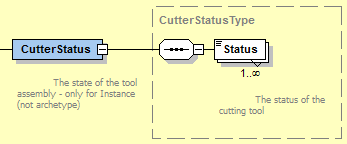
\includegraphics[width=1.0\textwidth]{figures/cutterstatus-schema.png}
  }
  \caption{CutterStatus Schema}
  \label{fig:cutterstatus-schema}
\end{figure}

\FloatBarrier

The elements of the \gls{cutterstatus} element can be a combined set of \gls{status cutterstatus} elements.  The \gls{mtconnect standard} allows any set of statuses to be combined, but only certain combinations make sense.  A \gls{cuttingtool} \SHOULD not be both \gls{new status} and \gls{used status} at the same time.  There are no rules in the schema to enforce this, but this is left to the implementer.  The following combinations \MUSTNOT occur: 

\begin{itemize}
    \item \gls{new status} \MUSTNOT be used with \gls{used status}, \gls{reconditioned status}, or \gls{expired status}.
    \item \gls{unknown status} \MUSTNOT be used with any other status. 
    \item \gls{allocated status} and \gls{unallocated status} \MUSTNOT be used together.
    \item \gls{available value} and \gls{unavailable value} \MUSTNOT be used together.
    \item If the tool is \gls{expired status}, \gls{broken status}, or \gls{notregistered status} it \MUSTNOT be \gls{available value}.
    \item All other combinations are allowed.
\end{itemize}


\tabulinesep = 5pt
\begin{longtabu} to \textwidth {
    |l|X[3l]|X[0.75l]|}
\caption{Elements for CutterStatus} \label{table:elements-for-cutterstatus} \\

\hline
Element & Description & Occurrence \\
\hline
\endfirsthead

\hline
\multicolumn{3}{|c|}{Continuation of Table \ref{table:elements-for-cutterstatus}}\\
\hline
Element & Description & Occurrence \\
\hline
\endhead

\gls{status cutterstatus}
&
\glsentrydesc{status cutterstatus}
 There can be multiple \gls{status cutterstatus} elements.
&
1..* \\
\hline


\end{longtabu}



\subparagraph{Status Element for CutterStatus} \mbox{}

One of the values for the status of the \gls{cuttingtool}.

\tabulinesep = 5pt
\begin{longtabu} to \textwidth {
    |l|X[0.75l]|}
\caption{Values for Status Element of CutterStatus} \label{table:values-for-status} \\

\hline
Value & Description\\
\hline
\endfirsthead

\hline
\multicolumn{2}{|c|}{Continuation of Table \ref{table:values-for-status}}\\
\hline
Value & Description\\
\hline
\endhead

\gls{new status}
&
\glsentrydesc{new status}
\\
\hline

\gls{available value}
&
Indicates the tool is available for use. If this is not present, the tool is currently not ready to be used.
\\
\hline

\gls{unavailable value}
&
Indicates the tool is unavailable for use in metal removal. If this is not present, the tool is currently not ready to be used.
\\
\hline

\gls{allocated status}
&
\glsentrydesc{allocated status}
\\
\hline

\gls{unallocated status}
&
\glsentrydesc{unallocated status}
\\
\hline

\gls{measured status}
&
\glsentrydesc{measured status}
\\
\hline

\gls{reconditioned status}
&
\glsentrydesc{reconditioned status}
\\
\hline

\gls{used status}
&
\glsentrydesc{used status}
\\
\hline

\gls{expired status}
&
\glsentrydesc{expired status}
\\
\hline

\gls{broken status}
&
\glsentrydesc{broken status}
\\
\hline

\gls{notregistered status}
&
\glsentrydesc{notregistered status}
\\
\hline

\gls{unknown status}
&
\glsentrydesc{unknown status}
\\
\hline


\end{longtabu}

\pagebreak

\paragraph{ToolLife Element for CuttingToolLifeCycle}\mbox{}

\begin{figure}[ht]
  \centering
  \scalebox{0.5}{
  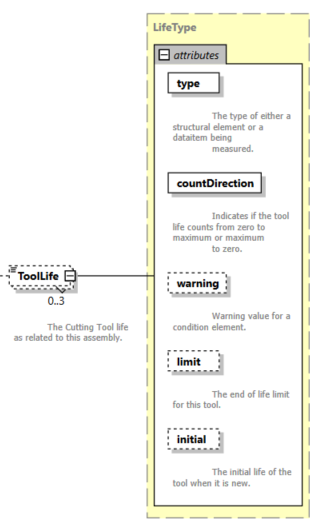
\includegraphics[width=1.0\textwidth]{figures/toollife-schema.png}
  }
  \caption{ToolLife Schema}
  \label{fig:toollife-schema}
\end{figure}

\FloatBarrier

The value is the current value for the \gls{toollife}.  The value \MUST be a number.  \gls{toollife} is an option element which can have three types, either minutes for time based, part count for parts based, or wear based using a distance measure.  One \gls{toollife} element can appear for each type, but there cannot be two entries of the same type.  Additional types can be added in the future.

\pagebreak

\subparagraph{Attributes for ToolLife}\mbox{}

\gls{toollife} has the following attributes that can be used to indicate the behavior of the tool life management mechanism.

\tabulinesep = 5pt
\begin{longtabu} to \textwidth {
    |l|X[3l]|X[0.75l]|}
\caption{Attributes for ToolLife} \label{table:attributes-for-toollife} \\

\hline
Attribute & Description & Occurrence \\
\hline
\endfirsthead

\hline
\multicolumn{3}{|c|}{Continuation of Table \ref{table:attributes-for-toollife}}\\
\hline
Attribute & Description & Occurrence \\
\hline
\endhead

\gls{type}
&
The type of tool life being accumulated. \gls{minutes type}, \gls{partcount}, or \gls{wear type}.
\newline \gls{type} is a required attribute.
&
1 \\
\hline
 
\gls{countdirection}
&
\glsentrydesc{countdirection}
 The value \MUST be one of \gls{up value} or \gls{down value}.
\newline \gls{countdirection} is a required attribute.
&
1 \\
\hline

\gls{warning toollife}
&
\glsentrydesc{warning toollife}
\newline \gls{warning toollife} is an optional attribute.
&
0..1 \\
\hline

\gls{limit}
&
The end of life limit for this tool. If the \gls{countdirection} is \gls{down value}, the point at which this tool should be expired, usually zero. If the \gls{countdirection} is \gls{up value}, this is the upper limit for which this tool should be expired.
\newline \gls{limit} is an optional attribute.
&
0..1 \\
\hline

\gls{initial}
&
The initial life of the tool when it is new.
\newline \gls{initial} is an optional attribute.
&
0..1 \\
\hline


\end{longtabu}

\subparagraph{type Attribute for ToolLife}\mbox{}

The value of \gls{type} must be one of the following:

\tabulinesep = 5pt
\begin{longtabu} to \textwidth {
    |l|X[0.75l]|}
\caption{Values for type of ToolLife}
\label{table:values-for-type-toollife} \\

\hline
Value & Description\\
\hline
\endfirsthead

\hline
\multicolumn{2}{|c|}{Continuation of Table \ref{table:values-for-type-toollife}}\\
\hline
Value & Description\\
\hline
\endhead

\gls{minutes type}
&
\glsentrydesc{minutes type}
\\
\hline

\gls{partcount}
&
The tool life measured in parts. All units for minimum, maximum, and nominal \MUST be provided as the number of parts.
\\
\hline

\gls{wear type}
&
\glsentrydesc{wear type}
 The standard will only consider dimensional wear at this time.
\\
\hline


\end{longtabu}

\subparagraph{countDirection Attribute for ToolLife}\mbox{}

The value of \gls{countdirection} must be one of the following:

\tabulinesep = 5pt
\begin{longtabu} to \textwidth {
    |l|X[0.75l]|}
\caption{Values for countDirection}
\label{table:values-for-countdirection-toollife} \\

\hline
Value & Description\\
\hline
\endfirsthead

\hline
\multicolumn{2}{|c|}{Continuation of Table \ref{table:values-for-countdirection-toollife}}\\
\hline
Value & Description\\
\hline
\endhead

\gls{up value}
&
The tool life counts up from zero to the maximum.
\\
\hline

\gls{down value}
&
The tool life counts down from the maximum to zero.
\\
\hline


\end{longtabu}

\paragraph{Location Element for CuttingToolLifeCycle}\mbox{}

\begin{figure}[ht]
  \centering
  \scalebox{0.5}{
  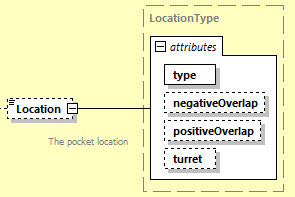
\includegraphics[width=1.0\textwidth]{figures/location-schema.png}
  }
  \caption{Location Schema}
  \label{fig:location-schema}
\end{figure}

\FloatBarrier

\gls{location} element identifies the specific location where a tool resides in a piece of equipment tool storage or in a tool crib.  This can be any series of numbers and letters as defined by the \gls{xml} type \gls{nmtoken}.  When a \gls{pot type} or \gls{station type} type is used, the value \MUST be a numeric value.  If a \gls{negativeoverlap} or the \gls{positiveoverlap} is provided, the tool reserves additional locations on either side, otherwise if they are not given, no additional locations are required for this tool.  If the pot occupies the first or last location, a rollover to the beginning or the end of the index-able values may occur.  For example, if there are 64 pots and the tool is in pot 64 with a \gls{positiveoverlap} of 1, the first pot \MAY be occupied as well.

\subparagraph{Attributes for Location}\mbox{}

\tabulinesep = 5pt
\begin{longtabu} to \textwidth {
    |l|X[3l]|X[0.75l]|}
\caption{Attributes for Location} \label{table:attributes-for-location} \\

\hline
Attribute & Description & Occurrence \\
\hline
\endfirsthead

\hline
\multicolumn{3}{|c|}{Continuation of Table \ref{table:attributes-for-location}}\\
\hline
Attribute & Description & Occurrence \\
\hline
\endhead

\gls{type}
&
The type of location being identified.
\newline \gls{type} \MUST be one of \gls{pot type}, \gls{station type}, or \gls{crib type}.
\newline \gls{type} is a required attribute.
&
1 \\
\hline
 
\gls{positiveoverlap}
&
\glsentrydesc{positiveoverlap}
\newline \gls{positiveoverlap} is a optional attribute.
&
0..1 \\
\hline

\gls{negativeoverlap}
&
\glsentrydesc{negativeoverlap}
\newline \gls{negativeoverlap} is an optional attribute.
&
0..1 \\
\hline


\end{longtabu}

\subparagraph{type Attribute for Location}\mbox{}

The type of location being identified.

\tabulinesep = 5pt
\begin{longtabu} to \textwidth {
    |l|X[0.75l]|}
\caption{Values for type of Location}
\label{table:values-for-type-location} \\

\hline
Value & Description\\
\hline
\endfirsthead

\hline
\multicolumn{2}{|c|}{Continuation of Table \ref{table:values-for-type-location}}\\
\hline
Value & Description\\
\hline
\endhead

\gls{pot type}
&
\glsentrydesc{pot type}
\\
\hline

\gls{station type}
&
\glsentrydesc{station type}
\\
\hline

\gls{crib type}
&
\glsentrydesc{crib type}
\\
\hline


\end{longtabu}

\subparagraph{postiveOverlap Attribute for Location}\mbox{}

The number of locations at higher index values that the \gls{cuttingtool} occupies due to interference.	 The value \MUST be an integer.  If not provided it is assumed to be 0. 

\subparagraph{negativeOverlap Attribute for Location}\mbox{}

The number of locations at lower index values that the \gls{cuttingtool} occupies due to interference. The value \MUST be an integer.  If not provided it is not assumed to be 0.

The tool number assigned in the part program and is used for cross referencing this tool information with the process parameters.	 The value \MUST be an integer.

\paragraph{ReconditionCount Element for CuttingToolLifeCycle}\mbox{}

\begin{figure}[ht]
  \centering
  \scalebox{0.7}{
  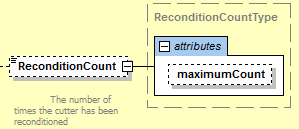
\includegraphics[width=1.0\textwidth]{figures/reconditioncount-schema.png}
  }
  \caption{ReconditionCount Schema}
  \label{fig:reconditioncount-schema}
\end{figure}

\FloatBarrier

This element \MUST contain an integer value as the \gls{cdata} that represents the number of times the cutter has been reconditioned. 

\subparagraph{Attributes for ReconditionCount}\mbox{}

\tabulinesep = 5pt
\begin{longtabu} to \textwidth {
    |l|X[3l]|X[0.75l]|}
\caption{Attributes for ReconditionCount} \label{table:attributes-for-reconditioncount} \\

\hline
Attribute & Description & Occurrence \\
\hline
\endfirsthead

\hline
\multicolumn{3}{|c|}{Continuation of Table \ref{table:attributes-for-reconditioncount}}\\
\hline
Attribute & Description & Occurrence \\
\hline
\endhead

\gls{maximumcount}
&
\glsentrydesc{maximumcount}
\newline \gls{maximumcount} is a optional attribute.
&
0..1 \\
\hline


\end{longtabu}

\pagebreak

\subsubsection{CuttingToolArchetypeReference Element for Cutting Tool}\mbox{}

\begin{figure}[ht]
  \centering
  \scalebox{0.7}{
  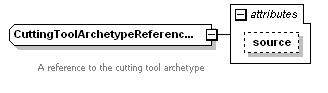
\includegraphics[width=1.0\textwidth]{figures/cuttingtoolarchetypereference-schema.png}
  }
  \caption{CuttingToolArcheTypeReference Schema}
  \label{fig:cuttingtoolarchetypereference-schema}
\end{figure}

\FloatBarrier

This optional element references another \gls{mtconnect asset} document providing the static geometries and nominal values for all the measurements. This reduces the amount of data duplication as well as providing a mechanism for asset definitions to be provided before complete measurement has occurred.

\paragraph{source Attribute for CuttingToolArcheTypeReference}\mbox{}

\tabulinesep = 5pt
\begin{longtabu} to \textwidth {
    |l|X[3l]|X[0.75l]|}
\caption{Attributes for CuttingToolArchetypeReference} \label{table:attributes-for-cuttingtoolarchetypereference} \\

\hline
Attribute & Description & Occurrence \\
\hline
\endfirsthead

\hline
\multicolumn{3}{|c|}{Continuation of Table \ref{table:attributes-for-cuttingtoolarchetypereference}}\\
\hline
Attribute & Description & Occurrence \\
\hline
\endhead

\gls{source attribute}
&
The URL of the \gls{cuttingtoolarchetype} \gls{information model}.
\newline This \MUST be a fully qualified URL as in http://example.com/asset/A213155
&
0..1 \\
\hline

\end{longtabu}

\section{Common Entity CuttingToolLifeCycle}
\label{sec:Common Entity CuttingToolLifeCycle}

\subsection{CuttingToolLifeCycle}
\label{sec:CuttingToolLifeCycle}

The life cycle refers to the data pertaining to the application or the use of the tool.  This data is provided by various pieces of equipment (i.e. machine tool, presetter) and statistical process control applications.  Life cycle data will not remain static, but will change periodically when a tool is used or measured.  The life cycle has three conceptual parts; \gls{cuttingtool} and \gls{cuttingitem} identity, properties, and measurements.  A measurement is defined as a constrained value that is reported in defined units and as a W3C floating point format.

The \gls{cuttingtoollifecycle} contains data for the entire tool assembly.  The specific \glspl{cuttingitem} that are part of the \gls{cuttingtoollifecycle} are contained in the \glspl{cuttingitem} element.  Each Cutting Item has similar properties as the assembly; identity, properties, and \glspl{measurement}.

The units for all \glspl{measurement} have been predefined in the \gls{mtconnect standard} and will be consistent with \citetitle{MTCPart2} and \citetitle{MTCPart3}.  This means that all lengths and distances will be given in millimeters and all angular measures will be given in degrees.  Quantities like \gls{processspindlespeed} will be given in RPM, the same as the \gls{rotaryvelocity sample} in \citetitle{MTCPart3}.

\subsubsection{XML Schema Structure for CuttingToolLifeCycle}

The \gls{cuttingtoollifecycle} schema shown in \fig{cuttingtoollifecycle-schema} is used in both the \gls{cuttingtoolarchetype} and \gls{cuttingtool} \glspl{information model}.  The only difference is that the elements \gls{cutterstatus}, \gls{toollife}, \gls{location}, and \gls{reconditioncount} are used only in the \gls{cuttingtool} \gls{information model}.

\begin{figure}[ht]
  \centering
  \scalebox{.4}{
  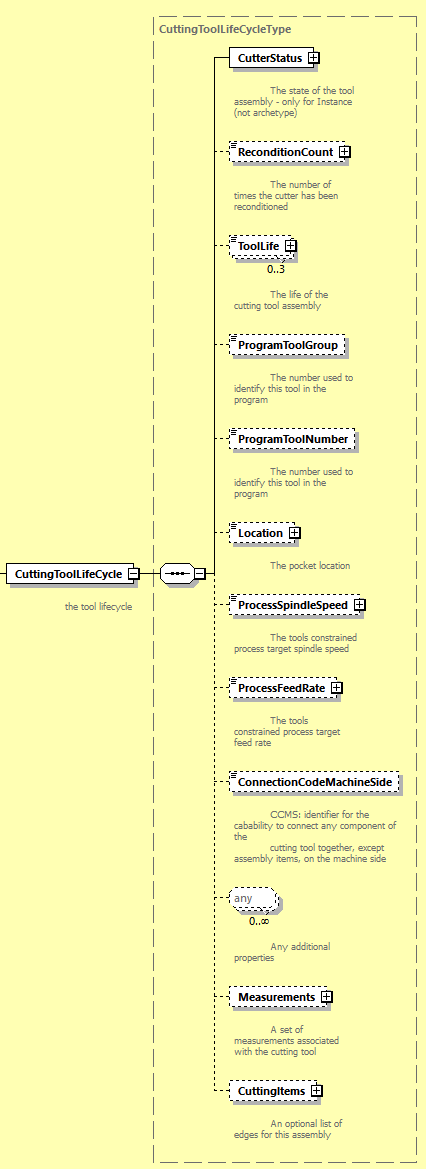
\includegraphics[width=1\textwidth]{figures/cuttingtoollifecycle-schema.png}}
  \caption{CuttingToolLifeCycle Schema}
  \label{fig:cuttingtoollifecycle-schema}
\end{figure}

\FloatBarrier

\subsection{Elements for CuttingToolLifeCycle}

The elements associated with this Cutting Tool are given in \tbl{elements-for-cuttingtoollifecycle}. The elements \MUST be provided in the following order as prescribed by XML.


\tabulinesep = 5pt
\begin{longtabu} to \textwidth {
    |l|X[2l]|X[0.75l]|}
\caption{Elements for CuttingToolLifeCycle} \label{table:elements-for-cuttingtoollifecycle} \\

\hline
Element & Description & Occurrence \\
\hline
\endfirsthead

\hline
\multicolumn{3}{|c|}{Continuation of Table \ref{table:elements-for-cuttingtoollifecycle}}\\
\hline
Element & Description & Occurrence \\
\hline
\endhead

\gls{cutterstatus}	
&
\glsentrydesc{cutterstatus}
\newline \gls{cutterstatus} can be one of the following values:
\gls{new status}, \gls{available value}, \gls{unavailable value}, \gls{allocated status}, \gls{unallocated status}, \gls{measured status}, \gls{reconditioned status}, \gls{notregistered status}, \gls{used status}, \gls{expired status}, \gls{broken status}, or \gls{unknown status}.
\newline \MUST only be used in the \gls{cuttingtool} \gls{information model}.
&
1 \\
\hline

\gls{reconditioncount}	
&
\glsentrydesc{reconditioncount}
\newline \MUST only be used in the \gls{cuttingtool} \gls{information model}.
&
0..1 \\
\hline

\gls{toollife}	
&
\glsentrydesc{toollife}
\newline \MUST only be used in the \gls{cuttingtool} \gls{information model}.
&
0..1 \\
\hline

\gls{location}	
&
\glsentrydesc{location}
\newline \MUST only be used in the \gls{cuttingtool} \gls{information model}.
&
0..1 \\
\hline

\gls{programtoolgroup}	
&
\glsentrydesc{programtoolgroup}
&
0..1 \\
\hline

\gls{programtoolnumber}	
&
\glsentrydesc{programtoolnumber}
&
0..1 \\
\hline

\gls{processspindlespeed}	
&
\glsentrydesc{processspindlespeed}
&
0..1 \\
\hline

\gls{processfeedrate}	
&
\glsentrydesc{processfeedrate}
&
0..1 \\
\hline

\gls{connectioncodemachineside}	
&
\glsentrydesc{connectioncodemachineside}
&
0..1 \\
\hline

\gls{measurements}	
&
A collection of measurements for the tool assembly. 
&
0..1 \\
\hline

\gls{cuttingitems}	
&
An optional set of individual Cutting Items.
&
0..1 \\
\hline

\gls{xs:any}	
&
\glsentrydesc{xs:any}
&
0..n \\
\hline


\end{longtabu}



\subsubsection{ProgramToolGroup Element for CuttingToolLifeCycle}

The optional identifier for the group of Cutting Tools when multiple tools can be used interchangeably. This is defined as an XML string type and is implementation dependent. 

\subsubsection{ProgramToolNumber Element for CuttingToolLifeCycle}

The tool number assigned in the part program and is used for cross referencing this tool information with the process parameters. The value \MUST be an integer.

\pagebreak 

\subsubsection{ProcessSpindleSpeed Element for CuttingToolLifeCycle}

\begin{figure}[ht]
  \centering
  \scalebox{.7}{
  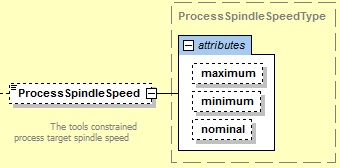
\includegraphics[width=1.0\textwidth]{figures/processspindlespeed-schema.png}
  }
  \caption{ProcessSpindleSpeed Schema}
  \label{fig:processspindlespeed-schema}
\end{figure}

\FloatBarrier

The \gls{processspindlespeed} \MUST be specified in revolutions/minute (RPM).  The \gls{cdata} \MAY contain the nominal process target spindle speed if available.  The maximum and minimum speeds \MAY be provided as attributes.  If \gls{processspindlespeed} is provided, at least one value of \gls{maximum attribute}, \gls{nominal attribute}, or \gls{minimum attribute} \MUST be specified.

\paragraph{Attributes for ProcessSpindleSpeed}\mbox{}

\tabulinesep = 5pt
\begin{longtabu} to \textwidth {
    |l|X[3l]|X[0.75l]|}
\caption{Attributes for ProcessSpindleSpeed} \label{table:attributes-for-processspindlespeed} \\

\hline
Attribute & Description & Occurrence \\
\hline
\endfirsthead

\hline
\multicolumn{3}{|c|}{Continuation of Table \ref{table:attributes-for-processspindlespeed}}\\
\hline
Attribute & Description & Occurrence \\
\hline
\endhead

\gls{maximum attribute}
&
The upper bound for the tool’s target spindle speed.
\newline \gls{maximum attribute} is an optional attribute.
&
0..1 \\
\hline
 
\gls{minimum attribute}
&
The lower bound for the tools spindle speed.
\newline \gls{minimum attribute} is a optional attribute.
&
0..1 \\
\hline

\gls{nominal attribute}
&
The nominal speed the tool is designed to operate at.
\newline \gls{nominal attribute} is an optional attribute.
&
0..1 \\
\hline


\end{longtabu}

\clearpage

\subsubsection{ProcessFeedRate Element for CuttingToolLifeCycle}

\begin{figure}[ht]
  \centering
  \scalebox{.7}{
  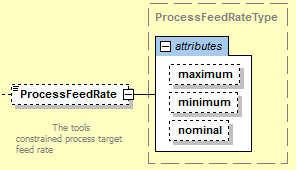
\includegraphics[width=1.0\textwidth]{figures/processfeedrate-schema.png}
  }
  \caption{ProcessFeedRate Schema}
  \label{fig:processfeedrate-schema}
\end{figure}

\FloatBarrier

The \gls{processfeedrate} \MUST be specified in millimeters/second (mm/s).  The \gls{cdata} \MAY contain the nominal process target feed rate if available.  The maximum and minimum rates MAY be provided as attributes.  If \gls{processfeedrate} is provided, at least one value of \gls{maximum attribute}, \gls{nominal attribute}, or \gls{minimum attribute} \MUST be specified.

\paragraph{Attributes for ProcessFeedRate}\mbox{}

\tabulinesep = 5pt
\begin{longtabu} to \textwidth {
    |l|X[3l]|X[0.75l]|}
\caption{Attributes for ProcessFeedRate} \label{table:attributes-for-processfeedrate} \\

\hline
Attribute & Description & Occurrence \\
\hline
\endfirsthead

\hline
\multicolumn{3}{|c|}{Continuation of Table \ref{table:attributes-for-processfeedrate}}\\
\hline
Attribute & Description & Occurrence \\
\hline
\endhead

\gls{maximum attribute}
&
The upper bound for the tool’s process target feedrate.
\newline \gls{maximum attribute} is an optional attribute.
&
0..1 \\
\hline
 
\gls{minimum attribute}
&
The lower bound for the tools feedrate.
\newline \gls{minimum attribute} is a optional attribute.
&
0..1 \\
\hline

\gls{nominal attribute}
&
The nominal feedrate the tool is designed to operate at.
\newline \gls{nominal attribute} is an optional attribute.
&
0..1 \\
\hline


\end{longtabu}


\subsubsection{ConnectionCodeMachineSide Element for CuttingToolLifeCycle}

This is an optional identifier for implementation specific connection component of the Cutting Tool on the machine side.  Code: \cfont{CCMS}.  The \gls{cdata} \MAY be any valid string according to the referenced connection code standards.

\subsubsection{xs:any Element for CuttingToolLifeCycle}

Utilizing the new capability in \gls{xml schema} Version 1.1, there are extension points where an additional element can be added to the document without being part of a substitution group.  The new elements have the restriction that they \MUSTNOT be part of the \gls{mtconnect} \gls{namespace} and \MUSTNOT be one of the predefined elements mentioned above.

This allows one to add additional properties to the \gls{cuttingtool} without having to change the definition of the \gls{cuttingtool} or modify the standard. The new capabilities were introduced in Version 1.3 of the \gls{mtconnect standard} and necessitate using Version 1.1 of \gls{xml schema} to make use of this form of extensible properties. 

\subsubsection{Measurements Element for CuttingToolLifeCycle}

The \glspl{measurement} element is a collection of one or more constrained scalar values associated with this Cutting Tool.  The \gls{xml} element \MUST be a type extension of the base types \gls{commonmeasurement} or \gls{assemblymeasurement}.  The following section defines the abstract \gls{measurement} type used in both \gls{cuttingtoollifecycle} and \gls{cuttingitem}.  This subsequent sections describe the \gls{assemblymeasurement} types followed by the \gls{cuttingitemmeasurement} types.

A \gls{measurement} is specific to the tool management policy at a particular shop.  The tool zero reference point or gauge line will be different depending on the particular implementation and will be assumed to be consistent within the shop.  \gls{mtconnect standard} does not standardize the manufacturing process or the definition of the zero point. 

\pagebreak

\subsubsection{Measurement}

\begin{figure}[ht]
  \centering
  \scalebox{0.5}{
  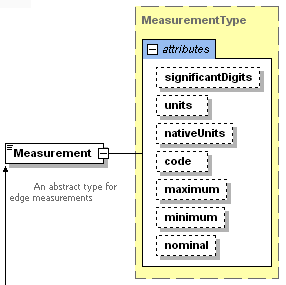
\includegraphics[width=1.0\textwidth]{figures/measurement-schema.png}
  }
  \caption{Measurement Schema}
  \label{fig:measurement-schema}
\end{figure}

\FloatBarrier

A \gls{measurement} \MUST be a scalar floating-point value that \MAY be constrained to a maximum and minimum value.  Since the \gls{cuttingtoollifecycle}’s main responsibility is to track aspects of the tool that change over its use in the shop, \gls{mtconnect} represents the current value of the \gls{measurement} \MUST be in the \gls{cdata} (text between the start and end element) as the most current valid value.

The \gls{minimum attribute} and \gls{maximum attribute} \MAY be supplied if they are known or relevant to the \gls{measurement}.  A \gls{nominal attribute} value \MAY be provided to show the reference value for this \gls{measurement}.

There are three abstract subtypes of  \gls{measurement}: \gls{commonmeasurement}, \gls{assemblymeasurement}, and \gls{cuttingitemmeasurement}.  These abstract types \MUSTNOT appear in an \gls{mtconnectassets} document, but are used in the schema as a way to separate which measurements \MAY appear in the different sections of the document.  Only subtypes that have extended these types \MAY appear in the \gls{mtconnectassets} XML.

\Glspl{measurement} in the \gls{cuttingtoollifecycle} section \MUST refer to the entire assembly and not to an individual \gls{cuttingitem}. \gls{cuttingitem} measurements \MUST be located in the measurements associated with the individual \gls{cuttingitem}.

\Glspl{measurement}  \MAY provide an optional \gls{units} attribute to reinforce the given units.  The units \MUST always be given in the predefined MTConnect units.  If \gls{units} are provided, they are only for documentation purposes.  \gls{nativeunits} \MAY optionally be provided to indicate the original units provided for the measurements. 

\paragraph{Attributes for Measurement}\mbox{}

\tabulinesep = 5pt
\begin{longtabu} to \textwidth {
    |l|X[3l]|X[0.75l]|}
\caption{Attributes for Measurement} \label{table:attributes-for-measurement} \\

\hline
Attribute & Description & Occurrence \\
\hline
\endfirsthead

\hline
\multicolumn{3}{|c|}{Continuation of Table \ref{table:attributes-for-measurement}}\\
\hline
Attribute & Description & Occurrence \\
\hline
\endhead

\gls{code measurement}
&
\glsentrydesc{code measurement}
\newline \gls{code measurement} is a optional attribute.
&
0..1 \\
\hline
 
\gls{maximum attribute}
&
The maximum value for this measurement. Exceeding this
value would indicate the tool is not usable.
\newline \gls{maximum attribute} is a optional attribute.
&
0..1 \\
\hline

\gls{minimum attribute}
&
The minimum value for this measurement. Exceeding this
value would indicate the tool is not usable.
\newline \gls{minimum attribute} is a optional attribute.
&
0..1 \\
\hline

\gls{nominal attribute}
&
The as advertised value for this measurement.
\newline \gls{nominal attribute} is a optional attribute.
&
0..1 \\
\hline

\gls{significantdigits}
&
The number of significant digits in the reported value. This is used by applications to determine accuracy of values. This \MAY be specified for all numeric values.
\newline \gls{significantdigits} is a optional attribute.
&
0..1 \\
\hline

\gls{units}
&
The units for the measurements. MTConnect Standard defines all the units for each measurement, so this is mainly for documentation sake. See MTConnect \citetitle{MTCPart2} 7.2.2.5 for the full list of units.
\newline \gls{units} is a optional attribute.
&
0..1 \\
\hline

\gls{nativeunits}
&
The units the measurement was originally recorded in. This is only necessary if they differ from units. See \citetitle{MTCPart2} Section 7.2.2.6 for the full list of units.
\newline \gls{nativeunits} is a optional attribute.
&
0..1 \\
\hline


\end{longtabu}

\paragraph{Measurement Subtypes for CuttingToolLifeCycle}\mbox{}

These \glspl{measurement} for \gls{cuttingtool} are specific to the entire assembly and \MUSTNOT be used for the \gls{measurement}  pertaining to a \gls{cuttingitem}. \fig{cutting-tool-measurement-1} and \fig{cutting-tool-measurement-2} will be used to reference the assembly specific \glspl{measurement}.

The Code in \tbl{measurement-subtypes-for-cuttingtool} will refer to the acronyms in the diagrams. We will be referring to many diagrams to disambiguate all measurements of the \gls{cuttingtool} and \gls{cuttingitem}. 

\begin{figure}[ht]
  \centering
  \scalebox{0.7}{
  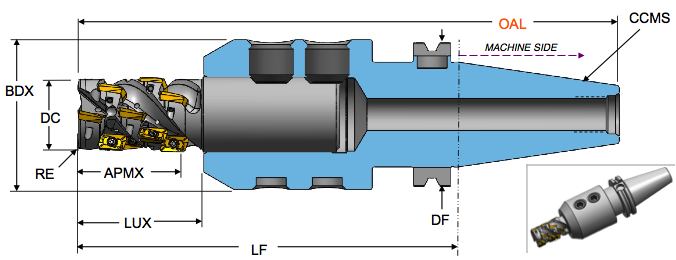
\includegraphics[width=1.0\textwidth]{figures/cutting-tool-measurement-1.png}
  }
  \caption{Cutting Tool Measurement Diagram 1}
  \label{fig:cutting-tool-measurement-1}
\end{figure}

\FloatBarrier

\begin{figure}[ht]
  \centering
  \scalebox{0.7}{
  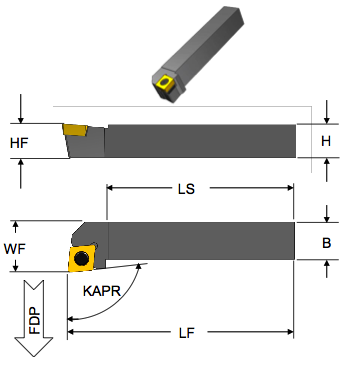
\includegraphics[width=1.0\textwidth]{figures/cutting-tool-measurement-2.png}
  }
  \caption{Cutting Tool Measurement Diagram 2}
  \label{fig:cutting-tool-measurement-2}
\end{figure}

\FloatBarrier

\tabulinesep = 5pt
\begin{longtabu} to \textwidth {
    |l|l|X[3l]|l|}
\caption{Measurement Subtypes for CuttingTool} \label{table:measurement-subtypes-for-cuttingtool} \\

\hline
Measurement Subtype & Code & Description & Units \\
\hline
\endfirsthead

\hline
\multicolumn{4}{|c|}{Continuation of Table \ref{table:measurement-subtypes-for-cuttingtool}}\\
\hline
Measurement Subtype & Code & Description & Units \\
\hline
\endhead

\gls{bodydiametermax} & \glscode{bodydiametermax} & \glsentrydesc{bodydiametermax} & \glsunits{bodydiametermax}
\\ \hline

\gls{bodylengthmax} & \glscode{bodylengthmax} & \glsentrydesc{bodylengthmax} & \glsunits{bodylengthmax}
\\ \hline

\gls{depthofcutmax} & \glscode{depthofcutmax} & \glsentrydesc{depthofcutmax} & \glsunits{depthofcutmax}
\\ \hline

\gls{cuttingdiametermax} & \glscode{cuttingdiametermax} & \glsentrydesc{cuttingdiametermax} & \glsunits{cuttingdiametermax}
\\ \hline

\gls{flangediametermax} & \glscode{flangediametermax} & \glsentrydesc{flangediametermax} & \glsunits{flangediametermax}
\\ \hline

\gls{overalltoollength} & \glscode{overalltoollength} & \glsentrydesc{overalltoollength} & \glsunits{overalltoollength}
\\ \hline

\gls{shankdiameter} & \glscode{shankdiameter} & \glsentrydesc{shankdiameter} & \glsunits{shankdiameter}
\\ \hline

\gls{shankheight} & \glscode{shankheight} & \glsentrydesc{shankheight} & \glsunits{shankheight}
\\ \hline

\gls{shanklength} & \glscode{shanklength} & \glsentrydesc{shanklength} & \glsunits{shanklength}
\\ \hline

\gls{usablelengthmax} & \glscode{usablelengthmax} & \glsentrydesc{usablelengthmax} & \glsunits{usablelengthmax}
\\ \hline

\gls{protrudinglength} & \glscode{protrudinglength} & \glsentrydesc{protrudinglength} & \glsunits{protrudinglength}
\\ \hline

\gls{weight} & \glscode{weight} & \glsentrydesc{weight} & \glsunits{weight}
\\ \hline

\gls{functionallength} & \glscode{functionallength} & \glsentrydesc{functionallength} & \glsunits{functionallength}
\\ \hline

\end{longtabu}

\subsubsection{CuttingItems Element for CuttingToolLifeCycle}

\begin{figure}[ht]
  \centering
  \scalebox{.5}{
  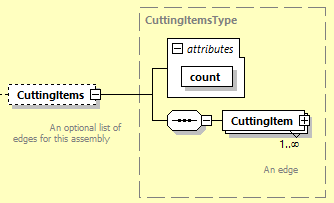
\includegraphics[width=1.0\textwidth]{figures/cuttingitems-schema.png}
  }
  \caption{CuttingItems Schema}
  \label{fig:cuttingitems-schema}
\end{figure}

\FloatBarrier

An optional collection of \glspl{cuttingitem} that \SHOULD be provided for each independent edge or insert.  If the \glspl{cuttingitem} are not present; it indicates there is no specific information with respect to each of the \glspl{cuttingitem}.  This does not imply there are no \glspl{cuttingitem} – there \MUST be at least one \gls{cuttingitem} – but there is no specific information.

\paragraph{Attributes for CuttingItems}\mbox{}

\tabulinesep = 5pt
\begin{longtabu} to \textwidth {
    |l|X[3l]|X[0.75l]|}
\caption{Attributes for CuttingItems} \label{table:attributes-for-cuttingitems} \\

\hline
Attribute & Description & Occurrence \\
\hline
\endfirsthead

\hline
\multicolumn{3}{|c|}{Continuation of Table \ref{table:attributes-for-cuttingitems}}\\
\hline
Attribute & Description & Occurrence \\
\hline
\endhead

\gls{count model}
&
The number of Cutting Item.
\newline \gls{count model} is a required attribute.
&
1 \\
\hline


\end{longtabu}


\subsubsection{CuttingItem}

A \gls{cuttingitem} is the portion of the tool that physically removes the material from the workpiece by shear deformation.  The Cutting Item can be either a single piece of material attached to the \gls{cuttingitem} or it can be one or more separate pieces of material attached to the \gls{cuttingitem} using a permanent or removable attachment.  A \gls{cuttingitem} can be comprised of one or more cutting edges.  \glspl{cuttingitem} include: replaceable inserts, brazed tips and the cutting portions of solid \glspl{cuttingtool}.

MTConnect Standard considers \glspl{cuttingitem} as part of the \gls{cuttingtool}.  A \glspl{cuttingitem} \MUSTNOT exist in MTConnect unless it is attached to a \gls{cuttingtool}.  Some of the measurements, such as \gls{functionallength}, \MUST be made with reference to the entire \gls{cuttingtool} to be meaningful.  

\begin{figure}[ht]
  \centering
  \scalebox{.5}{
  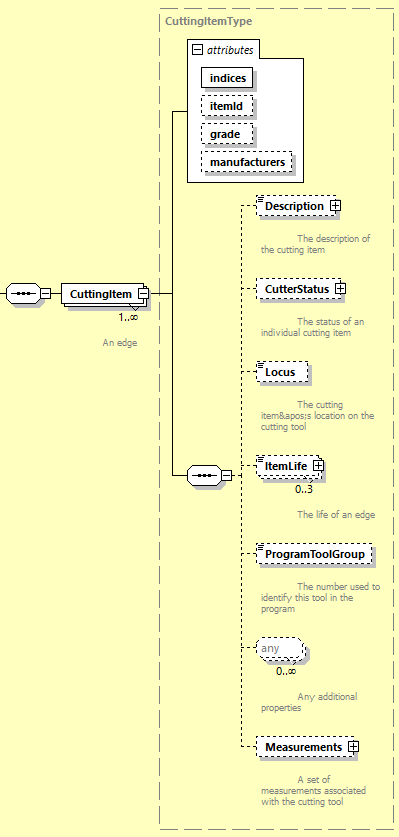
\includegraphics[width=1\textwidth]{figures/cuttingitem-schema.png}
  }
  \caption{CuttingItem Schema}
  \label{fig:cuttingitem-schema}
\end{figure}

\FloatBarrier

\paragraph{Attributes for CuttingItem}\mbox{}

\tabulinesep = 5pt
\begin{longtabu} to \textwidth {
    |l|X[3l]|X[0.75l]|}
\caption{Attributes for CuttingItem} \label{table:attributes-for-cuttingitem} \\

\hline
Attribute & Description & Occurrence \\
\hline
\endfirsthead

\hline
\multicolumn{3}{|c|}{Continuation of Table \ref{table:attributes-for-cuttingitem}}\\
\hline
Attribute & Description & Occurrence \\
\hline
\endhead

\gls{indices cuttingitem}
&
\glsentrydesc{indices cuttingitem}
\newline \gls{indices cuttingitem} is a required attribute.
&
1 \\
\hline


\gls{itemid cuttingitem}
&
\glsentrydesc{itemid cuttingitem}
\newline \gls{itemid cuttingitem} is an optional attribute.
&
0..1 \\
\hline

\gls{manufacturers}
&
\glsentrydesc{manufacturers}
\newline \gls{manufacturers} is an optional attribute.
&
0..1 \\
\hline

\gls{grade cuttingitem}
&
\glsentrydesc{grade cuttingitem}
\newline \gls{grade cuttingitem} is an optional attribute.
&
0..1 \\
\hline

\end{longtabu}

\subparagraph{indices Attribute for CuttingItem}\mbox{}

An identifier that indicates the \gls{cuttingitem} or \glspl{cuttingitem} these data are associated with.  The value \MUST be a single number ("1") or a comma separated set of individual elements ("1,2,3,4"), or as a inclusive range of values as in ("1-10") or any combination of ranges and numbers as in "1-4,6-10,22".  There \MUSTNOT be spaces or non-integer values in the text representation. 

Indices \SHOULD start numbering with the inserts or \gls{cuttingitem} furthest from the gauge line and increasing in value as the items get closer to the gauge line. Items at the same distance \MAY be arbitrarily numbered.

\subparagraph{itemId Attribute for CuttingItem}\mbox{}

The manufactures’ identifier for this \gls{cuttingitem} that \MAY be its catalog or reference number.  The value \MUST be an XML \gls{nmtoken} value of numbers and letters.

\subparagraph{manufacturers Attribute for CuttingItem}\mbox{}

This optional element references the manufacturers of this tool.  At this level the manufacturers will reference the \gls{cuttingitem} specifically.  The representation will be a comma (,) delimited list of manufacturer names.  This can be any series of numbers and letters as defined by the XML type \cfont{string}.

\subparagraph{grade Attribute for CuttingItem}\mbox{}

This provides an implementation specific designation for the material composition of this \gls{cuttingitem}.

\paragraph{Elements for CuttingItem}\mbox{}


\tabulinesep = 5pt
\begin{longtabu} to \textwidth {
    |l|X[3l]|X[0.75l]|}
\caption{Elements for CuttingItem} \label{table:elements-for-cuttingitem} \\

\hline
Element & Description & Occurrence \\
\hline
\endfirsthead

\hline
\multicolumn{3}{|c|}{Continuation of Table \ref{table:elements-for-cuttingitem}}\\
\hline
Element & Description & Occurrence \\
\hline
\endhead

\gls{description}	
&
A free-form description of the Cutting Item.
&
0..1 \\
\hline

\gls{locus cuttingitem}	
&
\glsentrydesc{locus cuttingitem}
&
0..1 \\
\hline

\gls{itemlife cuttingitem}	
&
\glsentrydesc{itemlife cuttingitem}
&
0..3 \\
\hline

\glspl{measurement}	
&
A collection of measurements relating to this Cutting Item.
&
0..1 \\
\hline

\end{longtabu}



\subparagraph{Description Element for CuttingItem}\mbox{}

An optional free form text description of this \gls{cuttingitem}. 

\subparagraph{Locus Element for CuttingItem}\mbox{}

Locus represents the location of the \gls{cuttingitem} with respect to the Cutting Tool.  For clarity, the words \cfont{FLUTE}, \cfont{INSERT}, and \cfont{CARTRIDGE} \SHOULD be used to assist in noting the location of a \gls{cuttingitem}.  The \gls{locus cuttingitem} \MAY be any free form text, but \SHOULD adhere to the following rules: 

\begin{itemize}
    \item  The location numbering \SHOULD start at the furthest \gls{cuttingitem} (\#1) and work it’s way back to the Cutting Item closest to the gauge line. 
    \item Flutes \SHOULD be identified as such using the word \cfont{FLUTE}:. For example: 
    \tab \cfont{FLUTE}: 1, \cfont{INSERT}: 2 - would indicate the first flute and the second furthest insert from the end of the tool on that flute.
    \item Other designations such as \cfont{CARTRIDGE} \MAY be included, but should be identified using upper case and followed by a colon (:).
\end{itemize}

\subparagraph{ItemLife Element for CuttingItem}\mbox{}

\begin{figure}[ht]
  \centering
  \scalebox{0.5}{
  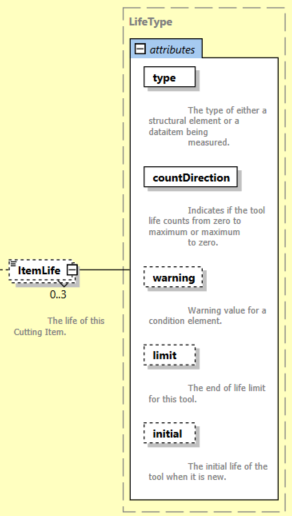
\includegraphics[width=1.0\textwidth]{figures/itemlife-schema.png}
  }
  \caption{ItemLife Schema}
  \label{fig:itemlife-schema}
\end{figure}

\FloatBarrier

The value is the current value for the \gls{toollife}.  The value \MUST be a number. \gls{toollife} is an option element which can have three types, either minutes for time based, part count for parts based, or wear based using a distance measure.  One tool life can appear for each type, but there cannot be two entries of the same type.  Additional types can be added in the future.

\subparagraph{Attributes for ItemLife}\mbox{}

These is an optional attribute that can be used to further classify the operation type.

\tabulinesep = 5pt
\begin{longtabu} to \textwidth {
    |l|X[3l]|X[0.75l]|}
\caption{Attributes for ItemLife} \label{table:attributes-for-itemlife} \\

\hline
Attribute & Description & Occurrence \\
\hline
\endfirsthead

\hline
\multicolumn{3}{|c|}{Continuation of Table \ref{table:attributes-for-itemlife}}\\
\hline
Attribute & Description & Occurrence \\
\hline
\endhead

\gls{type}
&
The type of tool life being accumulated. 
\newline \glspl{valid data value}:
\newline \gls{minutes type}, \gls{partcount}, or \gls{wear type}.
\newline \gls{type} is a required attribute.
&
1 \\
\hline
 
\gls{countdirection}
&
\glsentrydesc{countdirection}
The value \MUST be one of \gls{up value} or \gls{down value}.
\newline \gls{countdirection} is a required attribute.
&
1 \\
\hline

\gls{warning toollife}
&
\glsentrydesc{warning toollife}
\newline \gls{warning toollife} is an optional attribute.
&
0..1 \\
\hline

\gls{limit}
&
\glsentrydesc{limit}
\newline If the \gls{countdirection} is \gls{down value}, the point at which this tool should be expired, usually zero. If the \gls{countdirection} is \gls{up value}, this is the upper limit for which this tool should be expired.
\newline \gls{limit} is an optional attribute.
&
0..1 \\
\hline

\gls{initial}
&
\glsentrydesc{initial}
\newline \gls{initial} is an optional attribute.
&
0..1 \\
\hline


\end{longtabu}

\subparagraph{type Attribute for ItemLife}\mbox{}

The value of type must be one of the following:

\tabulinesep = 5pt
\begin{longtabu} to \textwidth {
    |l|X[0.75l]|}
\caption{Values for type of ItemLife}
\label{table:values-for-type-itemlife} \\

\hline
Value & Description\\
\hline
\endfirsthead

\hline
\multicolumn{2}{|c|}{Continuation of Table \ref{table:values-for-type-itemlife}}\\
\hline
Value & Description\\
\hline
\endhead

\gls{minutes type}
&
\glsentrydesc{minutes type}
\\
\hline

\gls{partcount}
&
The tool life measured in parts. All units for minimum, maximum, and nominal \MUST be provided as the number of parts.
\\
\hline

\gls{wear type}
&
\glsentrydesc{wear type}
\\
\hline


\end{longtabu}

\subparagraph{countDirection Attribute for ItemLife}\mbox{}

The value of type must be one of the following:

\tabulinesep = 5pt
\begin{longtabu} to \textwidth {
    |l|X[0.75l]|}
\caption{Values for countDirection}
\label{table:values-for-countdirection-itemlife} \\

\hline
Value & Description\\
\hline
\endfirsthead

\hline
\multicolumn{2}{|c|}{Continuation of Table \ref{table:values-for-countdirection-itemlife}}\\
\hline
Value & Description\\
\hline
\endhead

\gls{up value}
&
The tool life counts up from zero to the maximum.
\\
\hline

\gls{down value}
&
The tool life counts down from the maximum to zero.
\\
\hline


\end{longtabu}

\paragraph{Measurement Subtypes for CuttingItem}\mbox{}

These \glspl{measurement} for \gls{cuttingitem} are specific to an individual gls{cuttingitem} and \MUSTNOT be used for the  \glspl{measurement} pertaining to an assembly.  The \fig{cutting-tool}, \fig{cutting-item}, \fig{cutting-item-measurement-diagram-3} and \fig{cutting-item-drive-angle} will be used to for reference for the \gls{cuttingitem} specific \glspl{measurement} .

The Code in \tbl{measurement-subtypes-for-cuttingitem} will refer to the acronym in the diagram.  We will be referring to many diagrams to disambiguate all  \glspl{measurement} of the \glspl{cuttingtool} and \glspl{cuttingitem}.  We will present a few here; please refer to Appendix B for additional reference material.

\begin{figure}[ht]
  \centering
  \scalebox{0.7}{
  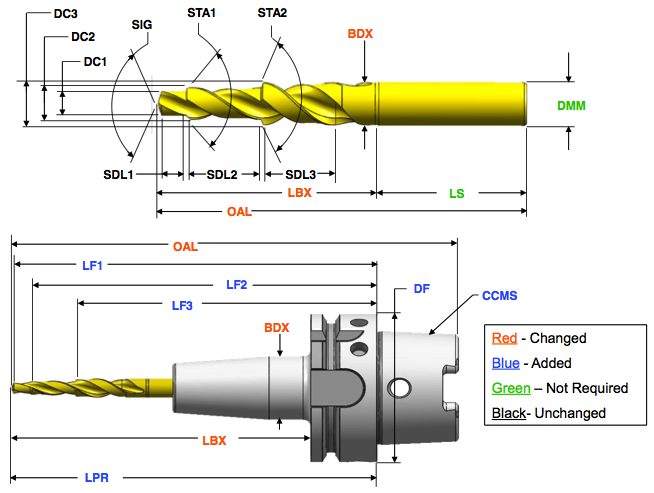
\includegraphics[width=1.0\textwidth]{figures/cutting-tool.png}
  }
  \caption{Cutting Tool}
  \label{fig:cutting-tool}
\end{figure}

\FloatBarrier

\begin{figure}[ht]
  \centering
  \scalebox{0.7}{
  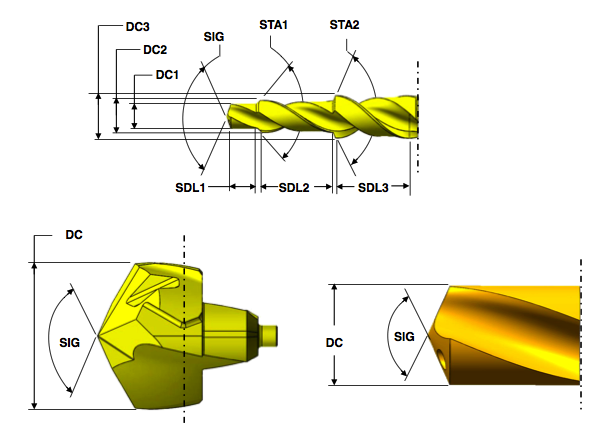
\includegraphics[width=1.0\textwidth]{figures/cutting-item.png}
  }
  \caption{Cutting Item}
  \label{fig:cutting-item}
\end{figure}

\FloatBarrier

\begin{figure}[ht]
  \centering
  \scalebox{0.7}{
  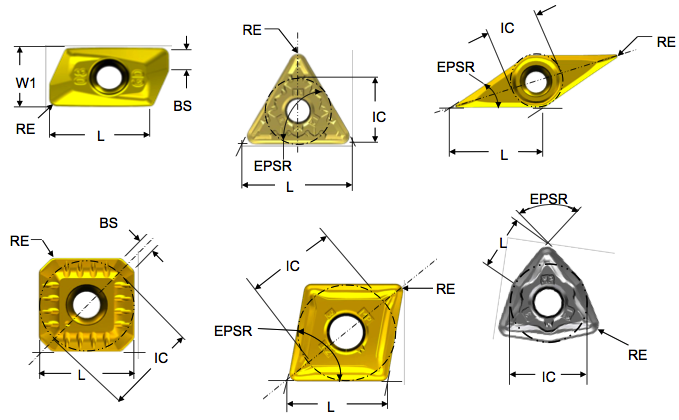
\includegraphics[width=1.0\textwidth]{figures/cutting-item-measurement-diagram-3.png}
  }
  \caption{Cutting Item Measurement Diagram 3}
  \label{fig:cutting-item-measurement-diagram-3}
\end{figure}

\FloatBarrier

\begin{figure}[ht]
  \centering
  \scalebox{0.3}{
  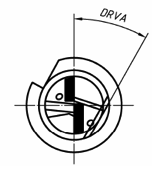
\includegraphics[width=1.0\textwidth]{figures/cutting-item-drive-angle.png}
  }
  \caption{Cutting Item Drive Angle}
  \label{fig:cutting-item-drive-angle}
\end{figure}

\FloatBarrier

The \gls{cuttingitem} \glspl{measurement} in \tbl{measurement-subtypes-for-cuttingitem} will refer the \fig{cutting-tool}, \fig{cutting-item}, \fig{cutting-item-measurement-diagram-3} and \fig{cutting-item-drive-angle}.

\tabulinesep = 5pt
\begin{longtabu} to \textwidth {
    |l|l|X[3l]|l|}
\caption{Measurement Subtypes for CuttingItem} \label{table:measurement-subtypes-for-cuttingitem} \\

\hline
Measurement Subtype & Code & Description & Units \\
\hline
\endfirsthead

\hline
\multicolumn{4}{|c|}{Continuation of Table \ref{table:measurement-subtypes-for-cuttingitem}}\\
\hline
Measurement Subtype & Code & Description & Units \\
\hline
\endhead

\gls{cuttingreferencepoint} & \glscode{cuttingreferencepoint} & \glsentrydesc{cuttingreferencepoint} & \glsunits{cuttingreferencepoint}
\\ \hline

\gls{cuttingedgelength} & \glscode{cuttingedgelength} & \glsentrydesc{cuttingedgelength} & \glsunits{cuttingedgelength}
\\ \hline

\gls{driveangle} & \glscode{driveangle} & \glsentrydesc{driveangle} & \glsunits{driveangle}
\\ \hline

\gls{flangediameter} & \glscode{flangediameter} & \glsentrydesc{flangediameter} & \glsunits{flangediameter}
\\ \hline

\gls{functionalwidth} & \glscode{functionalwidth} & \glsentrydesc{functionalwidth} & \glsunits{functionalwidth}
\\ \hline

\gls{incribedcirclediameter} & \glscode{incribedcirclediameter} & \glsentrydesc{incribedcirclediameter} & \glsunits{incribedcirclediameter}
\\ \hline

\gls{pointangle} & \glscode{pointangle} & \glsentrydesc{pointangle} & \glsunits{pointangle}
\\ \hline

\gls{toolcuttingedgeangle} & \glscode{toolcuttingedgeangle} & \glsentrydesc{toolcuttingedgeangle} & \glsunits{toolcuttingedgeangle}
\\ \hline

\gls{toolleadangle} & \glscode{toolleadangle} & \glsentrydesc{toolleadangle} & \glsunits{toolleadangle}
\\ \hline

\gls{toolorientation} & \glscode{toolorientation} & \glsentrydesc{toolorientation} & \glsunits{toolorientation}
\\ \hline

\gls{wiperedgelength} & \glscode{wiperedgelength} & \glsentrydesc{wiperedgelength} & \glsunits{wiperedgelength}
\\ \hline

\gls{stepdiameterlength} & \glscode{stepdiameterlength} & \glsentrydesc{stepdiameterlength} & \glsunits{stepdiameterlength}
\\ \hline

\gls{stepincludedangle} & \glscode{stepincludedangle} & \glsentrydesc{stepincludedangle} & \glsunits{stepincludedangle}
\\ \hline

\gls{cuttingdiameter} & \glscode{cuttingdiameter} & \glsentrydesc{cuttingdiameter} & \glsunits{cuttingdiameter}
\\ \hline

\gls{cuttingheight} & \glscode{cuttingheight} & \glsentrydesc{cuttingheight} & \glsunits{cuttingheight}
\\ \hline

\gls{cornerradius} & \glscode{cornerradius} & \glsentrydesc{cornerradius} & \glsunits{cornerradius}
\\ \hline

\gls{weight} & \glscode{weight} & \glsentrydesc{weight} & \glsunits{weight}
\\ \hline

\gls{functionallength cuttingitem} & \glscode{functionallength cuttingitem} & \glsentrydesc{functionallength cuttingitem} & \glsunits{functionallength cuttingitem}
\\ \hline

\gls{chamferflatlength} & \glscode{chamferflatlength} & \glsentrydesc{chamferflatlength} & \glsunits{chamferflatlength}
\\ \hline

\gls{chamferwidth} & \glscode{chamferwidth} & \glsentrydesc{chamferwidth} & \glsunits{chamferwidth}
\\ \hline

\gls{insertwidth} & \glscode{insertwidth} & \glsentrydesc{insertwidth} & \glsunits{insertwidth}
\\ \hline



\end{longtabu}
